%!TEX program = pdflatex

\documentclass{scrreprt}

\usepackage[autostyle]{csquotes}
\usepackage{amsmath}
\usepackage{graphicx}
\usepackage{gensymb}

\usepackage[
    backend=biber,
    style=authoryear-icomp,
    natbib=true,
    url=false, 
    doi=true,
    eprint=false
]{biblatex}
\addbibresource{bibtex.bib}

\usepackage[]{hyperref}
\hypersetup{
    colorlinks=true,
}

\usepackage[utf8]{inputenc}

%===================================================================================

\begin{document}

%!TEX root = structure.tex

\chapter{Introdução}\label{ch:introducao}

\section{}

Hello \citep{kendrew1958three}
%!TEX root = structure.tex

\chapter{Revisão de literatura}\label{ch:rev_literatura}


\section{Métodos de atribuição de estruturas secundárias}\label{section:metodos_atribuicao}
\input{rev_literatura/ss_atribuicao/intro}
\subsection{DSSP}

Em 1983, Kabsch e Sander publicaram o algoritmo de atribuição de estruturas secundárias de proteínas que viria a ser o mais utilizado até os dias atuais, o DSSP (\textit{Dictionary of Protein Secondary Structure}). 

No trabalho, os autores afirmam que a atribuição de estruturas secundárias a partir das coordenadas atômicas de estruturas proteicas é um problema de reconhecimento de padrões. Nesse contexto, eles optaram por identificar esses padrões através de ligações de hidrogênio entre átomos da cadeia principal ao invés de ângulos $\Phi$ e $\Psi$ ou de posições relativas de $C_\alpha$. A justificativa utilizada foi que a presença ou ausência de ligações de hidrogênio poderiam ser avaliadas por um simples critério energético, enquanto que outras características precisariam do ajuste de um número maior de parâmetros. %sidenote Na época havia um pouco mais de 100 estruturas depositadas

As ligações de hidrogênio foram definidas por eles utilizando um modelo eletrostático. Nesse modelo, uma ligação de hidrogênio $HB$ ocorrerá se, e somente se, a energia $E$ for menor que -0.5 kcal/mol. Para o cálculo são utilizadas as cargas parcias $+q_1, -q_1$ nos átomos $C$ e $O$, e $-q_2, +q_2$ nos átomos $N$ e $H$, onde $q_1=0.42e$ e $q_2=0.20e$.

\begin{gather}
E < -0.5 kcal/mol \implies HB = \text{Verdade}
\intertext{onde} 
E = q_1q_2(1/r(ON)+1/r(CH)-1/r(OH)-1/r(CN))*f \label{eq:dssp_energy}
\end{gather}

Na equação \eqref{eq:dssp_energy}, $r(AB)$ é a distância interatômica entre A e B em ângstroms e o fator dimensional $f=332$. 

Os autores afirmam que, por este modelo, uma boa ligação de hidrogênio teria aproximadamente -3 kcal/mol. Assim, a escolha de um limiar em -0.5 kcal/mol torna o modelo mais tolerante à erros nas coordenadas atômicas e à ligações de hidrogênios bifurcadas \citep{Kabsch1983}.

Uma vez definido o modelo para identificar ligações de hidrogênio, essas são testadas e anotadas na cadeia polipeptídica em duas classes elementares: (1) padrão \textit{n-Turn} e (2) padrão \textit{bridge}. 

O padrão \textit{n-Turn}, onde $n \in \{3, 4, 5\}$, apresentam uma ligação de hidrogênio entre o $CO$ do resíduo $i$ e o $NH$ do resíduo $i+n$.

% # Abstract

% Atribuição de estruturas secundárias através do reconhecimento de padrões de ligações de hidrogênio e características (features) geométricas extraídas de coordenadas de X-ray.

% Estruturas secundárias cooperativas são reconhecidas por repetições  de padrões de ligações de hidrogênio. Repetições de "turns" formam hélices, repetições de bridges formam "ladders", e "ladders" conectadas formam fitas.

% # Main Ideas

% Algoritmo baseado principalmente em padrões de ligações de hidrogênio. Requer o ajuste de um menor número de parâmetros em relação aos angulos phi e psi, ou as posições dos CA.

% Padrões:

% n-turns - (onde n pode ser 3,4 ou 5) apresentam uma ligação de hidrogênio entre o CO do resíduo i e o NH do resíduo i+n.

% bridges - ligações de hidrôgenio entre resíduos distantes na sequência.

% Esses dois padrões representam todos os possíveis padrões de ligações de hidrogênio entre átomos do backbone.

% Repetições de 4-turns definem uma alpha-hélice. Repetições de bridges definem uma estrutura beta. As outras ocorrências dos padrões básicos podem representar hélices-310, helices-pi, single turns e single beta-bridges.

% # Definições






\subsection{Stride}



stride
\subsection{KAKSI}

kaksi
\subsection{PROSS}

pross

\section{Métodos de predição de estruturas secundárias}
\subsection{Primeira geração (1957-1978)} 

primeira geraçao - chou e fasman - gor
\subsection{Segunda geração (1983-1992)} 

segunda geração - GORIII
\subsection{Terceira geração} 

terceira geração - aprendizado de máquina (NN) - PHDsec
\subsection{Quarta geração} 

quarta geração - aprendizado de máquina (NN) + dados evolutivos (PSSM) - PSIPred
\chapter{Resultados}

\section{Análise de métodos de atribuição de estrutura secundária}

Diferentemente de outros métodos de predição de estrutura secundária que utilizaram os resultados de atribuição provenientes de apenas um método, em geral o DSSP, nós optamos por utilizar os resultados de um concenso entre quatro métodos. Consequentemente, é importante analizar como esses métodos diferem entre si.

As diferenças entre as metologias de atribuição foram previamente discutidas na seção \ref{section:metodos_atribuicao}. Nesta seção, analisaremos as diferenças nas estruturas secundárias atribuídas aos resíduos.



\begin{figure}
  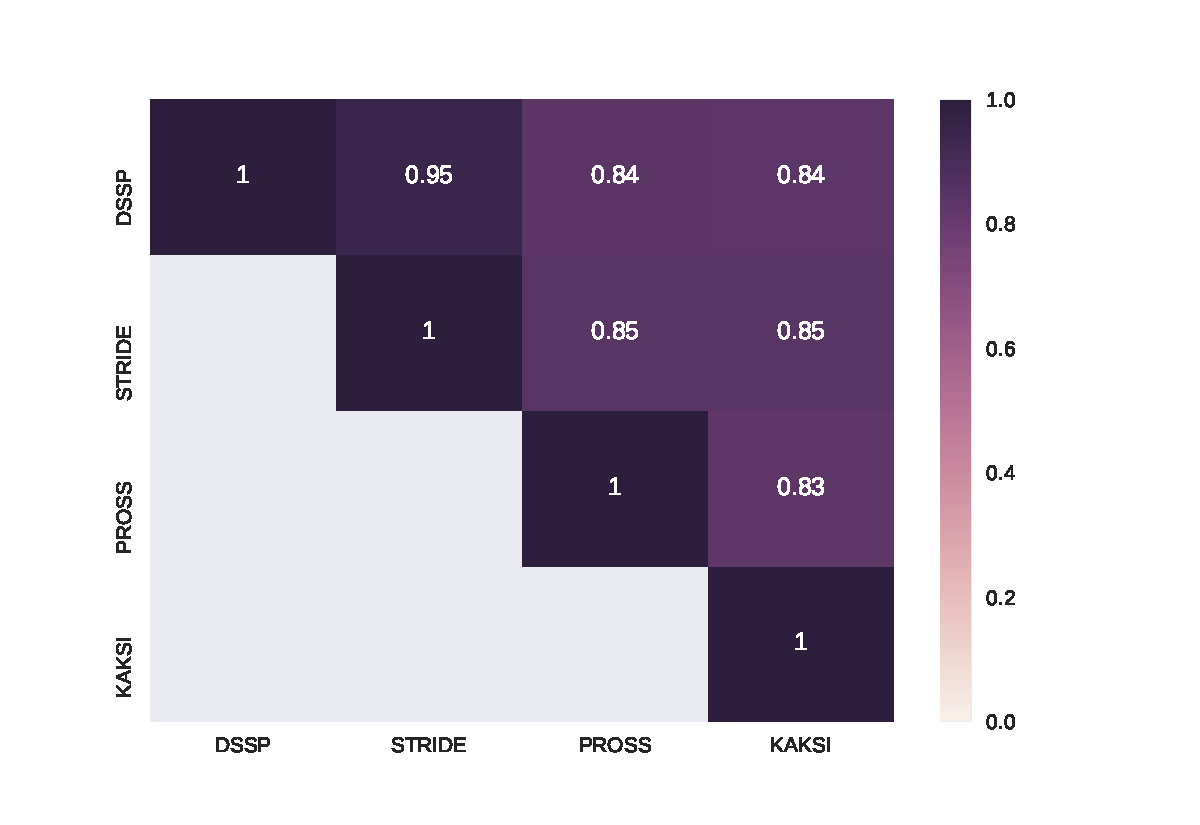
\includegraphics[width=\linewidth]{../figures/comparacao_metodos_atribuicao.pdf}
  \caption{Similaridade entre os métodos de atribuição de estruturas secundárias.}
  \label{fig:comparacao_metodos_atribuicao}
\end{figure}

\section{Resultados de predição com o PSIPRED}

O PSIPRED é um método de predição de estruturas secundárias que utiliza redes neurais artificias em conjunto com PSSM \citep{10.1006/jmbi.1999.3091} (ver \ref{ch:rev_literatura}). O método foi originalmente treinado com informações de estrutura secundária atribuídas pelo DSSP. 

Devido as variações observadas entre os métodos de atribuição de estrutura secundária, nós realizamos a comparação dos resultados de predição com a estrutura secundária atribuída por diferentes métodos, assim como com o consenso entre os métodos de atribuição.

No conjunto de proteínas utilizado nesse trabalho, o PSIPRED comparado à atribuição pelo DSSP, demonstrou uma acurácia média (Q3) de 86\%, superior aos 78\% descrito na literatura. 

A acurácia média para a predição de fitas $\beta$, como esperado, foi inferior a predição de hélices e coils.

Um resultado interessante foi a acurácia média observada entre a predição e o consenso dos métodos de atribuição estrutura secundária. Tanto a acurácia geral (Q3) quantos a acurácia por classe (Qh, Qe, Qc) demonstrou um aumento significativo em relação a comparação individual com os métodos de atribuição. 

Isso indica que para as regiões onde não há consenso entre os métodos de atribuição, a acurácia média (Q3) é próxima ou inferior a 68\%.

$Q3_\text{consenso}*P_\text{consenso} + Q3_\text{não consenso}*P_\text{não consenso} = Q3_\text{total}$

$Q3_\text{não consenso} = \frac{Q3_\text{total} - Q3_\text{consenso}*P_\text{consenso}}{P_\text{não consenso}}$

$Q3_\text{não consenso} = \frac{0.86 - 0.92*0.75}{0.25}$

$Q3_\text{não consenso} = 0.68$

%Comentar que entre os piores resultados de acurácia há grande presença de zinc fingers resolvidas em complexo com o DNA. Discutir o sentido disso

\begin{figure}
    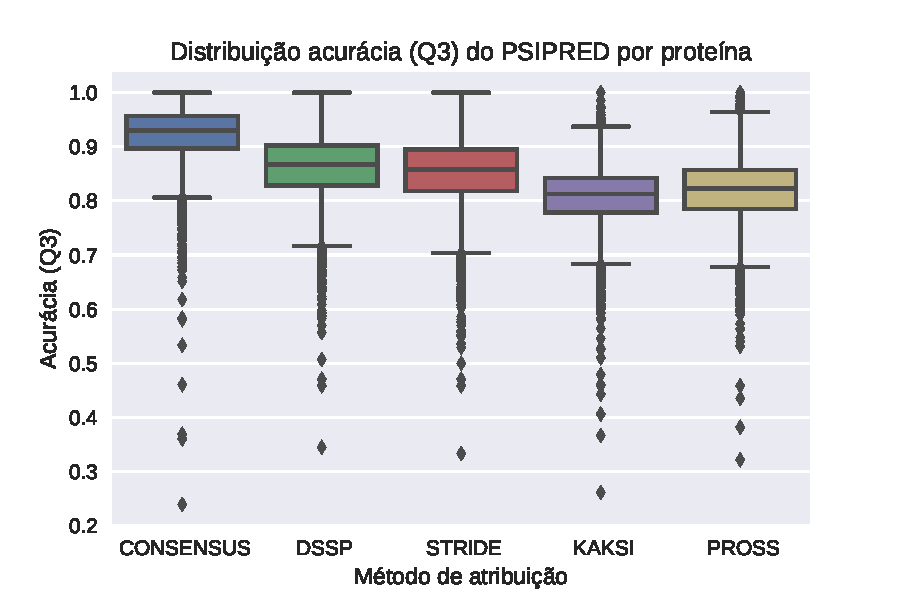
\includegraphics[width=\linewidth]{../figures/psipred_q3.pdf}
    \caption{}
    \label{fig:psipred_q3}
\end{figure}

\begin{figure}
    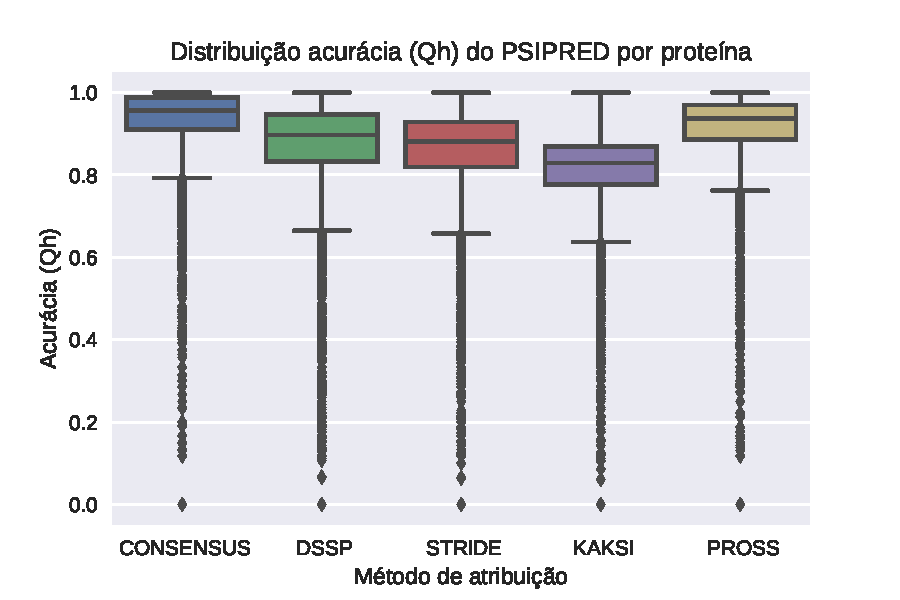
\includegraphics[width=\linewidth]{../figures/psipred_qh.pdf}
    \caption{}
    \label{fig:psipred_qh}
\end{figure}

\begin{figure}
    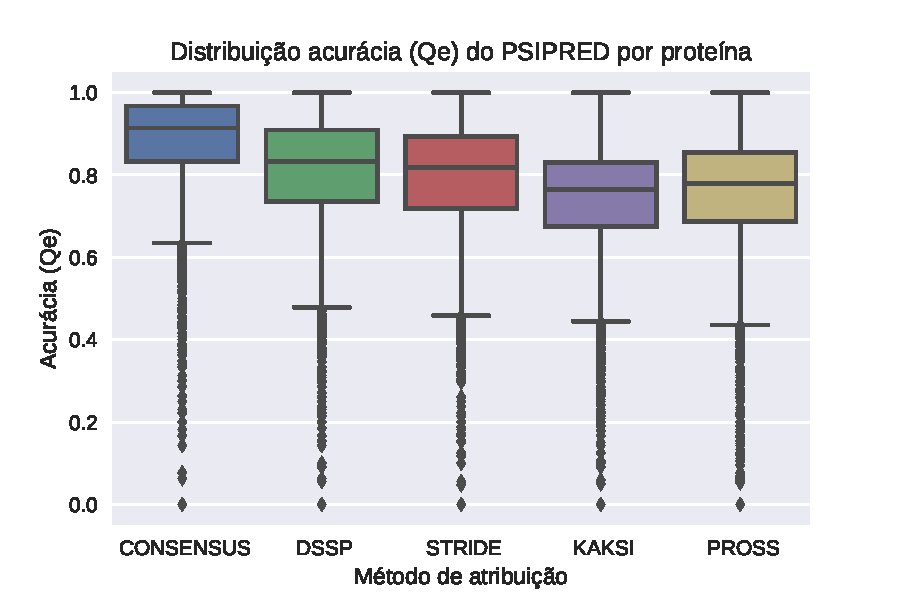
\includegraphics[width=\linewidth]{../figures/psipred_qe.pdf}
    \caption{}
    \label{fig:psipred_qe}
\end{figure}

\begin{figure}
    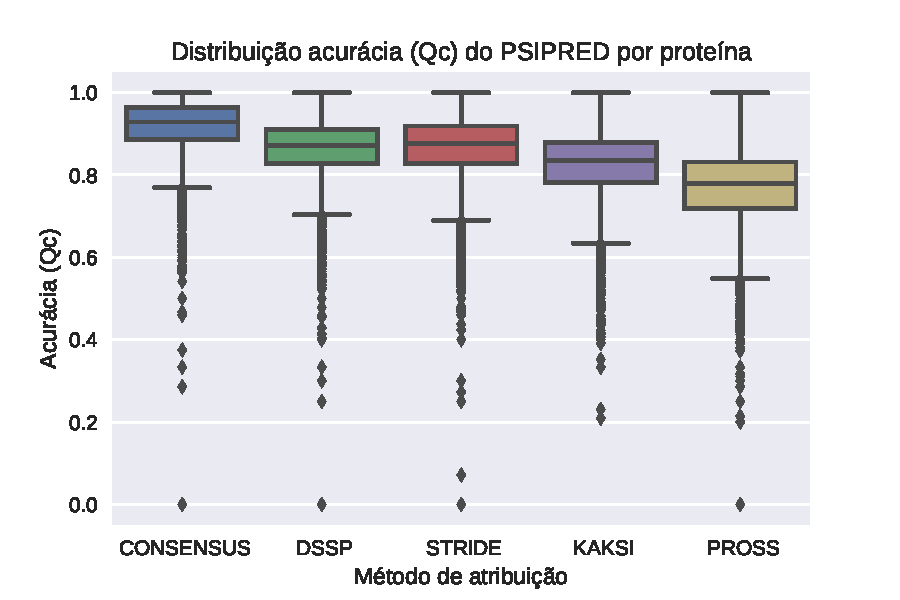
\includegraphics[width=\linewidth]{../figures/psipred_qc.pdf}
    \caption{}
    \label{fig:psipred_qc}
\end{figure}

\printbibliography 

\end{document}